\documentclass[a4paper, 12pt]{article}

\usepackage{cmap}
\usepackage[OT1]{fontenc}
\usepackage[utf8]{inputenc}
%\usepackage{mathtext}
%\usepackage{amsmath}
\usepackage[russian]{babel}
\usepackage{amsmath}
\usepackage{amsfonts}
\usepackage{amssymb}
\usepackage{graphicx}
%\usepackage[bookmarks=true, pdfpagemode=UseNone]{hyperref}
\usepackage{indentfirst}
\usepackage{listings}
%\usepackage{multicol}
%\usepackage{misccorr}
%\usepackage{longtable}
%\usepackage{flafter}
\usepackage{float}
%\usepackage{color}
%\usepackage{nccfloats}
%\usepackage{tabularx}
%\usepackage{graphicx}
%\usepackage[babel=true,protrusion=true,expansion=true]{microtype}
%\usepackage[left=1.8cm, right=1cm, top=1cm, bottom=1cm, bindingoffset=0cm]{geometry}

%\pagestyle{empty}

\author{Алексюк А.О., Мурашко Д.С.}
\title{Спектры простых сигналов}
\lstset{inputencoding=utf8, extendedchars=\true, keepspaces = true, language=Matlab}

\begin{document}
\maketitle
\tableofcontents
\pagebreak

\section{Цель работы}
Получить представление о свойствах спектров.

\section{Постановка задачи}
В командном окне MATLAB и в среде Simulink промоделировать следующие тестовые сигналы:
\begin{itemize}
\item Полигармонический сигнал
\item Прямоугольный импульсный сигнал
\item Треугольный импульсный сигнал
\end{itemize}
Получить спектров этих сигналов.

\section{Теоретическая часть}
\begin{itemize}
\item Полигармонический сигнал y(t)=$\sum\limits_{n=0}^{N-1} cos (nt)$ \newline
\item Прямоугольный импульсный сигнал y(t)=$\prod(t,Ti)$ \newline
\item Треугольный импульсный сигнал y(t)=$\Delta(t,Ti)$
\end{itemize}
\section{Ход работы}

\subsection{Код Matlab}
\begin{lstlisting}
close all;
clear all;
x = 0:0.01:4*pi;
f0 = 5;
%исходный сигнал
%for n=1:length(x)
%  y(n) = cos(2*pi*f0*n*x(n));
%end;
for n=1:length(x)
  if mod(n,20) < 10
      y(n) = 0;
  else
      y(n) = 1;
  end;
end;
y = conv(y,y);
for n=1:length(x)
    y(n) = y(n)/n;
end;
plot(x(1:200),y(1:200))
grid
%спектр исходного сигнала
figure
spectrum = fft(y,512);
norm_spectrum = spectrum.*conj(spectrum)/512;
f=100*(0:255)/512;
plot(f, norm_spectrum(1:256))
axis([0 max(f) 0 1000])
grid

\end{lstlisting}

\begin{figure}[H]
   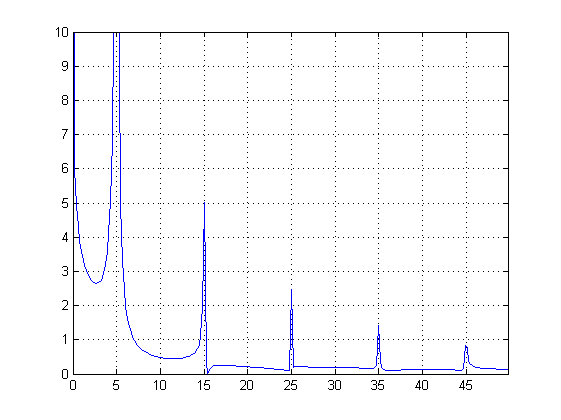
\includegraphics[scale=0.7]{lab5/1.png}
   \caption{Подписать}
\end{figure}

\begin{figure}[H]
   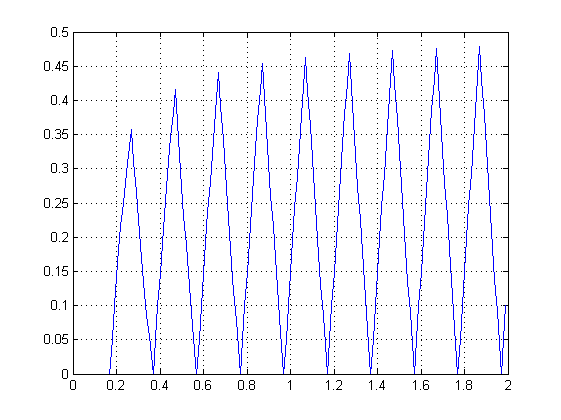
\includegraphics[scale=0.7]{lab5/2.png}
   \caption{Подписать}
\end{figure}

\subsection{Simulink}

\begin{figure}[H]
   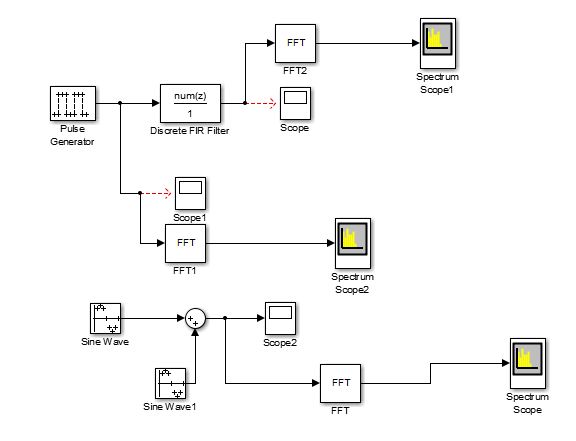
\includegraphics[scale=0.7]{lab5/simulink.png}
   \caption{Проект Simulink}
\end{figure}

\begin{figure}[H]
   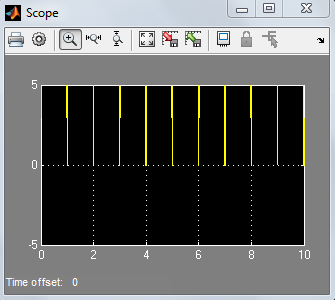
\includegraphics[scale=0.7]{lab5/scope.png}
   \caption{Подписать}
\end{figure}

\begin{figure}[H]
   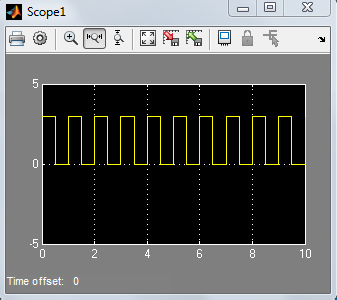
\includegraphics[scale=0.7]{lab5/scope1.png}
   \caption{Подписать}
\end{figure}
\begin{figure}[H]
   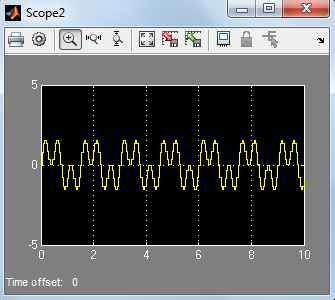
\includegraphics[scale=0.7]{lab5/scope2.png}
   \caption{Подписать}
\end{figure}


\section{Вывод}
В лабораторной работе было проведено моделирование полигармонического, прямоугольного и треугольного сигналаов. После чего получены их спектры. Треугольный сигнал представляет собой два участка прямых,
исходящих из одной точки - вершины, а интеграл от произведения двух констант есть линейная функция.
Поэтому треугольный сигнал был получен путем применения операции свертки для двух прямоугольных сигналов.  Данная операция осуществляется с помощью специальной функции Matlab. 
	

\end{document}